\حصہء{سوالات}
\موٹا{خطوط}\\
سوال \حوالہ{سوال_مخروط_خط_قطبی_کارتیسی_الف}  تا سوال \حوالہ{سوال_مخروط_خط_قطبی_کارتیسی_ت} میں دیے خطوط کی قطبی اور کارتیسی مساوات تلاش کریں۔ 

\ابتدا{سوال}\شناخت{سوال_مخروط_خط_قطبی_کارتیسی_الف}
خط شکل \حوالہ{شکل_سوال_مخروط_خط_قطبی_کارتیسی_الف} میں ترسیم کیا گیا ہے۔
\انتہا{سوال}
%========================
\ابتدا{سوال}\شناخت{سوال_مخروط_خط_قطبی_کارتیسی_ب}
خط شکل \حوالہ{شکل_سوال_مخروط_خط_قطبی_کارتیسی_ب} میں ترسیم کیا گیا ہے۔
\انتہا{سوال}
%========================
\ابتدا{سوال}\شناخت{سوال_مخروط_خط_قطبی_کارتیسی_پ}
خط شکل \حوالہ{شکل_سوال_مخروط_خط_قطبی_کارتیسی_پ} میں ترسیم کیا گیا ہے۔
\انتہا{سوال}
%========================
\ابتدا{سوال}\شناخت{سوال_مخروط_خط_قطبی_کارتیسی_ت}
خط شکل \حوالہ{شکل_سوال_مخروط_خط_قطبی_کارتیسی_ت} میں ترسیم کیا گیا ہے۔
\انتہا{سوال}
%========================
\begin{figure}
\centering
\begin{minipage}{0.22\textwidth}
\centering
\begin{tikzpicture}[font=\scriptsize]
\pgfmathsetmacro{\a}{30}
\pgfmathsetmacro{\d}{2}
\draw[-latex](-0.15,0)--(3,0)node[right]{$x$};
\draw[-latex](0,-0.15)--(0,2)node[above]{$y$};
\draw(0,0)--++(\a:\d)coordinate(ka)node[pos=0.5,above]{$5$};
\draw[thick](\a:\d)++(\a-90:1.5)coordinate(kb)--++(\a+90:2.5);
\RightAngle{(0,0)}{(ka)}{(kb)}
\draw[-stealth]([shift={(0:0.5)}]0,0) arc (0:\a:0.5)node[right,yshift=-1ex]{$\tfrac{\pi}{6}$};
\end{tikzpicture}
\caption{ترسیم سوال \حوالہ{سوال_مخروط_خط_قطبی_کارتیسی_الف}}
\label{شکل_سوال_مخروط_خط_قطبی_کارتیسی_الف}
\end{minipage}\hfill
\begin{minipage}{0.22\textwidth}
\centering
\begin{tikzpicture}[font=\scriptsize]
\pgfmathsetmacro{\a}{135}
\pgfmathsetmacro{\d}{2}
\draw[-latex](-2.5,0)--(0.5,0)node[right]{$x$};
\draw[-latex](0,-0.15)--(0,2)node[above]{$y$};
\draw(0,0)--++(\a:\d)coordinate(ka)node[pos=0.5,above]{$2$};
\draw[thick](\a:\d)++(\a-90:1.5)coordinate(kb)--++(\a+90:2.5);
\RightAngle{(0,0)}{(ka)}{(kb)}
\draw[-stealth]([shift={(0:0.3)}]0,0) arc (0:\a:0.3)node[pos=0.25,above]{$\tfrac{3\pi}{4}$};
\end{tikzpicture}
\caption{ترسیم سوال \حوالہ{سوال_مخروط_خط_قطبی_کارتیسی_ب}}
\label{شکل_سوال_مخروط_خط_قطبی_کارتیسی_ب}
\end{minipage}\hfill
\begin{minipage}{0.22\textwidth}
\centering
\begin{tikzpicture}[font=\scriptsize]
\pgfmathsetmacro{\a}{240}
\pgfmathsetmacro{\d}{2}
\draw[-latex](-0.5,0)--(0.5,0)node[right]{$x$};
\draw[-latex](0,-0.15)--(0,0.5)node[above]{$y$};
\draw(0,0)--++(\a:\d)coordinate(ka)node[pos=0.5,above]{$3$};
\draw[thick](\a:\d)++(\a-90:1.5)coordinate(kb)--++(\a+90:2.5);
\RightAngle{(0,0)}{(ka)}{(kb)}
\draw[-stealth]([shift={(0:0.3)}]0,0) arc (0:\a:0.3)node[pos=0.75,above left]{$\tfrac{4\pi}{3}$};
\end{tikzpicture}
\caption{ترسیم سوال \حوالہ{سوال_مخروط_خط_قطبی_کارتیسی_پ}}
\label{شکل_سوال_مخروط_خط_قطبی_کارتیسی_پ}
\end{minipage}\hfill
\begin{minipage}{0.22\textwidth}
\centering
\begin{tikzpicture}[font=\scriptsize]
\pgfmathsetmacro{\a}{-45}
\pgfmathsetmacro{\d}{2}
\draw[-latex](-0.15,0)--(2,0)node[right]{$x$};
\draw[-latex](0,-0.15)--(0,0.25)node[above]{$y$};
\draw(0,0)--++(\a:\d)coordinate(ka)node[pos=0.5,below]{$4$};
\draw[thick](\a:\d)++(\a-90:1.5)coordinate(kb)--++(\a+90:2.5);
\RightAngle{(0,0)}{(ka)}{(kb)}
\draw[-stealth]([shift={(0:0.3)}]0,0) arc (0:\a:0.3)node[pos=0.8,right]{$-\tfrac{\pi}{4}$};
\end{tikzpicture}
\caption{ترسیم سوال \حوالہ{سوال_مخروط_خط_قطبی_کارتیسی_ت}}
\label{شکل_سوال_مخروط_خط_قطبی_کارتیسی_ت}
\end{minipage}
\end{figure}

سوال \حوالہ{سوال_مخروط_قطبی_ترسیم_کارتیسی_معلوم_الف} تا سوال \حوالہ{سوال_مخروط_قطبی_ترسیم_کارتیسی_معلوم_ب} میں دی مساوات کو ترسیم کریں اور ان کی کارتیسی مساوات معلوم کریں۔ 

\ابتدا{سوال}\شناخت{سوال_مخروط_قطبی_ترسیم_کارتیسی_معلوم_الف}
$r\cos(\theta-\tfrac{\pi}{4})=\sqrt{2}$
\انتہا{سوال}
%======================
\ابتدا{سوال}
$r\cos(\theta+\tfrac{3\pi}{4})=1$
\انتہا{سوال}
%======================
\ابتدا{سوال}
$r\cos(\theta-\tfrac{2\pi}{3})=3$
\انتہا{سوال}
%======================
\ابتدا{سوال}\شناخت{سوال_مخروط_قطبی_ترسیم_کارتیسی_معلوم_ب}
$r\cos(\theta+\tfrac{\pi}{3})=2$
\انتہا{سوال}
%======================

سوال \حوالہ{سوال_مخروط_کارتیسی_سے_قطبی_معلوم_الف} تا سوال \حوالہ{سوال_مخروط_کارتیسی_سے_قطبی_معلوم_ب} میں دی گئی کارتیسی مساوات کی قطبی روپ (\عددی{r\cos(\theta-\theta_0)=r_0}) تلاش کریں۔ 

\ابتدا{سوال}\شناخت{سوال_مخروط_کارتیسی_سے_قطبی_معلوم_الف}
$\sqrt{2}x+\sqrt{2}y=6$
\انتہا{سوال}
%=======================
\ابتدا{سوال}
$\sqrt{3}x-y=1$
\انتہا{سوال}
%=======================
\ابتدا{سوال}
$y=-5$
\انتہا{سوال}
%=======================
\ابتدا{سوال}\شناخت{سوال_مخروط_کارتیسی_سے_قطبی_معلوم_ب}
$x=-4$
\انتہا{سوال}
%=======================

سوال \حوالہ{سوال_مخروط_دائرے_کی_قطبی_الف} تا سوال \حوالہ{سوال_مخروط_دائرے_کی_قطبی_ت} میں دی گئی دائروں کی قطبی مساوات دریافت کریں۔

\ابتدا{سوال}\شناخت{سوال_مخروط_دائرے_کی_قطبی_الف}
دائرہ شکل \حوالہ{شکل_سوال_مخروط_دائرے_کی_قطبی_الف}
\انتہا{سوال}
%========================
\ابتدا{سوال}\شناخت{سوال_مخروط_دائرے_کی_قطبی_ب}
دائرہ شکل \حوالہ{شکل_سوال_مخروط_دائرے_کی_قطبی_ب}
\انتہا{سوال}
%========================
\ابتدا{سوال}\شناخت{سوال_مخروط_دائرے_کی_قطبی_پ}
دائرہ شکل \حوالہ{شکل_سوال_مخروط_دائرے_کی_قطبی_پ}
\انتہا{سوال}
%========================
\ابتدا{سوال}\شناخت{سوال_مخروط_دائرے_کی_قطبی_ت}
دائرہ شکل \حوالہ{شکل_سوال_مخروط_دائرے_کی_قطبی_ت}
\انتہا{سوال}
%========================
\begin{figure}
\centering
\begin{minipage}{0.22\textwidth}
\centering
\begin{tikzpicture}[font=\scriptsize]
\draw[-latex](-0.15,0)--(2.5,0)node[right]{$x$};
\draw[-latex](0,-1)--(0,1)node[above]{$y$};
\draw(1,0)node[circ]{}  circle (1);
\draw(1,1)node[above]{رداس $=4$};
\end{tikzpicture}
\caption{دائرہ سوال \حوالہ{سوال_مخروط_دائرے_کی_قطبی_الف}}
\label{شکل_سوال_مخروط_دائرے_کی_قطبی_الف}
\end{minipage}\hfill
\begin{minipage}{0.22\textwidth}
\centering
\begin{tikzpicture}[font=\scriptsize]
\draw[-latex](-1,0)--(1,0)node[right]{$x$};
\draw[-latex](0,-2.25)--(0,0.25)node[above]{$y$};
\draw(0,-1)node[circ]{}  circle (1);
\draw(0,0)node[above right]{رداس $=1$};
\end{tikzpicture}
\caption{دائرہ سوال \حوالہ{سوال_مخروط_دائرے_کی_قطبی_ب}}
\label{شکل_سوال_مخروط_دائرے_کی_قطبی_ب}
\end{minipage}\hfill
\begin{minipage}{0.22\textwidth}
\centering
\begin{tikzpicture}[font=\scriptsize]
\draw[-latex](-1,0)--(1,0)node[right]{$x$};
\draw[-latex](0,-0.15)--(0,2.25)node[above]{$y$};
\draw(0,1)node[circ]{}  circle (1);
\draw(0,2)node[above right]{رداس $=\sqrt{2}$};
\end{tikzpicture}
\caption{دائرہ سوال \حوالہ{سوال_مخروط_دائرے_کی_قطبی_پ}}
\label{شکل_سوال_مخروط_دائرے_کی_قطبی_پ}
\end{minipage}\hfill
\begin{minipage}{0.22\textwidth}
\centering
\begin{tikzpicture}[font=\scriptsize]
\draw[-latex](-2.25,0)--(0.15,0)node[right]{$x$};
\draw[-latex](0,-1)--(0,1)node[above]{$y$};
\draw(-1,0)node[circ]{}  circle (1);
\draw(-1,1)node[above]{رداس $=\tfrac{1}{2}$};
\end{tikzpicture}
\caption{دائرہ سوال \حوالہ{سوال_مخروط_دائرے_کی_قطبی_ت}}
\label{شکل_سوال_مخروط_دائرے_کی_قطبی_ت}
\end{minipage}
\end{figure}

سوال \حوالہ{سوال_مخروط_قطبی_دائرے_ترسیم_الف} تا سوال \حوالہ{سوال_مخروط_قطبی_دائرے_ترسیم_ب} میں دیے گئے دائرے ترسیم کریں۔

\ابتدا{سوال}\شناخت{سوال_مخروط_قطبی_دائرے_ترسیم_الف}
$r=4\cos\theta$
\انتہا{سوال}
%=====================
\ابتدا{سوال}
$r=6\sin\theta$
\انتہا{سوال}
%=====================
\ابتدا{سوال}
$r=-2\cos\theta$
\انتہا{سوال}
%=====================
\ابتدا{سوال}\شناخت{سوال_مخروط_قطبی_دائرے_ترسیم_ب}
$r=-8\sin\theta$
\انتہا{سوال}
%=====================

سوال \حوالہ{سوال_مخروط_قطبی_پیچیدہ_الف} تا سوال \حوالہ{سوال_مخروط_قطبی_پیچیدہ_ب} کے قطبی مساوات معلوم کریں۔ 

\ابتدا{سوال}\شناخت{سوال_مخروط_قطبی_پیچیدہ_الف}
$(x-6)^2+y^2=36$
\انتہا{سوال}
%========================
\ابتدا{سوال}
$(x+2)^2+y^2=4$
\انتہا{سوال}
%========================
\ابتدا{سوال}
$x^2+(y-5)^2=25$
\انتہا{سوال}
%========================
\ابتدا{سوال}
$x^2+(y+7)^2=49$
\انتہا{سوال}
%========================
\ابتدا{سوال}
$x^2+2x+y^2=0$
\انتہا{سوال}
%========================
\ابتدا{سوال}
$x^2-16x+y^2=0$
\انتہا{سوال}
%========================
\ابتدا{سوال}
$x^2+y^2+y=0$
\انتہا{سوال}
%========================
\ابتدا{سوال}\شناخت{سوال_مخروط_قطبی_پیچیدہ_ب}
$x^2+y^2-\tfrac{4}{3}y=0$
\انتہا{سوال}
%========================

\موٹا{سنک اور ناظمہ سے مخروط خطے}

سوال \حوالہ{سوال_مخروط_سنک_ناظمہ_قطبی_الف} تا سوال \حوالہ{سوال_مخروط_سنک_ناظمہ_قطبی_ب} میں مخروط حصوں کی سنک دی گئی ہے۔ مخروط حصے کا ایک ماسکہ مبدا پر واقع ہے اور اس کا مطابقتی ناظمہ بھی دیا گیا ہے۔ اس مخروط حصے کی قطبی مساوات تلاش کریں۔

\ابتدا{سوال}\شناخت{سوال_مخروط_سنک_ناظمہ_قطبی_الف}
$e=1,\quad x=2$
\انتہا{سوال}
%=======================
\ابتدا{سوال}
$e=1,\quad y=2$
\انتہا{سوال}
%=======================
\ابتدا{سوال}
$e=5,\quad y=-6$
\انتہا{سوال}
%=======================
\ابتدا{سوال}
$e=2,\quad x=4$
\انتہا{سوال}
%=======================
\ابتدا{سوال}
$e=\tfrac{1}{2},\quad x=1$
\انتہا{سوال}
%=======================
\ابتدا{سوال}
$e=\tfrac{1}{4},\quad x=-2$
\انتہا{سوال}
%=======================
\ابتدا{سوال}
$e=\tfrac{1}{5},\quad y=-10$
\انتہا{سوال}
%=======================
\ابتدا{سوال}\شناخت{سوال_مخروط_سنک_ناظمہ_قطبی_ب}
$e=\tfrac{1}{3},\quad y=6$
\انتہا{سوال}
%=======================

\موٹا{قطع مکافی اور ترخیم}\\
سوال \حوالہ{سوال_مخروط_ترخیم_قطع_مکافی_الف} تا سوال \حوالہ{سوال_مخروط_ترخیم_قطع_مکافی_ب} کے قطع مکافی اور ترخیمات کو ترسیم کریں۔ مبدا پر واقع ماسکہ کا مطابقتی ناظمہ بھی ترسیم کریں۔ ہر مخروط حصے کی قطبی مساوات تلاش کریں۔

\ابتدا{سوال}\شناخت{سوال_مخروط_ترخیم_قطع_مکافی_الف}
$r=\tfrac{1}{1+\cos\theta}$
\انتہا{سوال}
%====================
\ابتدا{سوال}
$r=\tfrac{6}{2+\cos\theta}$
\انتہا{سوال}
%====================
\ابتدا{سوال}
$r=\tfrac{25}{1-5\cos\theta}$
\انتہا{سوال}
%====================
\ابتدا{سوال}
$r=\tfrac{4}{2-2\cos\theta}$
\انتہا{سوال}
%====================
\ابتدا{سوال}
$r=\tfrac{400}{16+8\sin\theta}$
\انتہا{سوال}
%====================
\ابتدا{سوال}
$r=\tfrac{12}{3+3\sin\theta}$
\انتہا{سوال}
%====================
\ابتدا{سوال}
$r=\tfrac{8}{2-2\sin\theta}$
\انتہا{سوال}
%====================
\ابتدا{سوال}\شناخت{سوال_مخروط_ترخیم_قطع_مکافی_ب}
$r=\tfrac{4}{2-\sin\theta}$
\انتہا{سوال}
%====================

\موٹا{عدم مساوات کی ترسیمات}\\

سوال \حوالہ{سوال_مخروط_عدم_مساوات_ترسیم_الف} اور سوال \حوالہ{سوال_مخروط_عدم_مساوات_ترسیم_ب} میں عدم مساوات کو ترسیم کریں۔

\ابتدا{سوال}\شناخت{سوال_مخروط_عدم_مساوات_ترسیم_الف}
$0\le r\le 2\cos\theta$
\انتہا{سوال}
%=====================
\ابتدا{سوال}\شناخت{سوال_مخروط_عدم_مساوات_ترسیم_ب}
$-3\cos\theta\le r\le 0$
\انتہا{سوال}
%=====================

\موٹا{کمپیوٹر کا استعمال}

سوال \حوالہ{سوال_مخروط_کمپیوٹر_خط_مخروط_الف} تا سوال \حوالہ{سوال_مخروط_کمپیوٹر_خط_مخروط_ب} میں دیے گئے خط اور مخروط خطے ترسیم کریں۔

\ابتدا{سوال}\شناخت{سوال_مخروط_کمپیوٹر_خط_مخروط_الف}
$r=3\sec(\theta-\tfrac{\pi}{3})$
\انتہا{سوال}
%=========================
\ابتدا{سوال}
$r=4\sec(\theta+\tfrac{\pi}{6})$
\انتہا{سوال}
%=========================
\ابتدا{سوال}
$r=4\sin\theta$
\انتہا{سوال}
%=========================
\ابتدا{سوال}
$r=-2\cos\theta$
\انتہا{سوال}
%=========================
\ابتدا{سوال}
$r=\tfrac{8}{4+\cos\theta}$
\انتہا{سوال}
%=========================
\ابتدا{سوال}
$r=\tfrac{8}{4+\sin\theta}$
\انتہا{سوال}
%=========================
\ابتدا{سوال}
$r=\tfrac{1}{1-\sin\theta}$
\انتہا{سوال}
%=========================
\ابتدا{سوال}
$r=\tfrac{1}{1+\cos\theta}$
\انتہا{سوال}
%=========================
\ابتدا{سوال}
$r=\tfrac{1}{1+2\sin\theta}$
\انتہا{سوال}
%=========================
\ابتدا{سوال}\شناخت{سوال_مخروط_کمپیوٹر_خط_مخروط_ب}
$r=\tfrac{1}{1+2\cos\theta}$
\انتہا{سوال}
%=========================

\موٹا{نظریہ اور مثالیں}\\
\ابتدا{سوال}\ترچھا{حضیض شمسی اور اوج شمسی}\\
ایک سیارہ اپنے سورج کے گرد ایک ترخیم پر گھومتا ہے جس کے نصف محور اکبر کی لمبائی \عددی{a} ہے۔
\begin{enumerate}[a.]
\item
دکھائیں کہ جب سیارہ سورج کے قریب تر ہو تب \عددی{r=a(1-e)} ہو گا اور جب یہ سورج سے دور تر ہو تب \عددی{r=a(1+e)} ہو گا۔
\item
جدول \حوالہ{جدول_مخروط_نظام_شمسی} کی مدد سے معلوم کریں کہ ہماری نظام شمسی میں ہر سیارہ سورج کے کتنے نزدیک اور اس سے کتنا دور ہو سکتا ہے۔
\end{enumerate}
\انتہا{سوال}
%====================
\begin{table}
\caption{نظام شمسی میں سیاروں کی سنک اور نصف محور اکبر}
\label{جدول_مخروط_نظام_شمسی}
\centering
\begin{tabular}{ccc}
\toprule
سیارہ& نصف محور اکبر (فلکی اکائیاں) & سنک\\
\midrule
عطارہ&$0.387$& $0.2056$\\
زھرہ&$0.7233$  & $0.0068$\\
زمین& $1.000$  &  $0.0167$\\
مریخ&  $1.524$  &  $0.0934$  \\
مشتری&  $5.203$   &  $0.0484$\\
زحل&  $9.539$  &  $0.0543$\\
یورانس&  $19.18$  &  $0.0460$\\
نیپچون&  $30.06$  &  $0.0082$\\
پلوٹو&  $39.44$   &  $0.2481$\\
\bottomrule
\end{tabular}
\end{table}
%===========================

\ابتدا{سوال}\ترچھا{سیاروں کی مدار پر حرکت}\\
ہم نے مثال \حوالہ{مثال_مخروط_مدار_پلوٹو} میں پلوٹو کے مدار کی قطبی مساوات معلوم کی۔ جدول \حوالہ{جدول_مخروط_نظام_شمسی} کی مدد سے دیگر سیاروں کے مدار کی مساوات تلاش کریں۔
\انتہا{سوال}
%=====================
\ابتدا{سوال}
(الف) منحنیات \عددی{r=4\sin\theta} اور \عددی{r=\sqrt{3}\sec\theta} کی کارتیسی مساواتیں تلاش کریں۔  (ب) ان دنوں منحنیات کو ایک ساتھ ترسیم کر کے ان کے نقطہ تقاطع کو کارتیسی اور قطبی محدد میں ظاہر کریں۔ 
\انتہا{سوال}
%=====================
\ابتدا{سوال}
(الف) منحنیات \عددی{r=8\cos\theta} اور \عددی{r=2\sec\theta} کی کارتیسی مساواتیں تلاش کریں۔  (ب) ان دنوں منحنیات کو ایک ساتھ ترسیم کر کے ان کے نقطہ تقاطع کو کارتیسی اور قطبی محدد میں ظاہر کریں۔ 
\انتہا{سوال}
%=======================
\ابتدا{سوال}
ایک قطع مکافی کا ماسکہ \عددی{(0,0)} پر ہے جبکہ اس کا ناظمہ \عددی{r\cos\theta=4} ہے۔ اس کی قطبی مساوات تلاش کریں۔
\انتہا{سوال}
%============================
\ابتدا{سوال}
ایک قطع مکافی کا ماسکہ \عددی{(0,0)} پر ہے جبکہ اس کا ناظمہ \عددی{r\cos(\theta-\tfrac{\pi}{2})=4} ہے۔ اس کی قطبی مساوات تلاش کریں۔
\انتہا{سوال}
%===========================
\ابتدا{سوال}\ترچھا{خلائی مہندس}\\
ترخیمی مدار کی سنک کا کلیہ خلائی مہندس درج ذیل لکھے گا
\begin{align*}
e=\frac{r_{\text{بلندتر}}-r_\text{\RL{کمتر}}}{r_{\text{بلندتر}}+r_\text{\RL{کمتر}}}
\end{align*}
جہاں خلائی جہاز سے قوت کشش کے مرکز تک فاصلہ \عددی{r} ہے۔ یہ کلیہ کیوں قابل استعمال ہے؟
\انتہا{سوال}
%================
\ابتدا{سوال}\ترچھا{ترخیم کی ترسیم بذریعہ دھاگہ}\\

\انتہا{سوال}
%=================
